\documentclass[fleqn]{article}
\usepackage{enumitem}
\usepackage{amsmath}
\usepackage{graphicx}
\usepackage{tikz-cd}
\usepackage[makeroom]{cancel}
\usepackage[paperheight=29.7cm, paperwidth=21.5cm, margin=3cm, top=3cm, bottom=2cm, left=3cm, right=2cm]{geometry}
\usepackage{array}
\usepackage{pgfplots}
\pgfplotsset{width=10cm,compat=1.9}

\newcommand{\jaw}{\\ \textbf{Jawaban} \\}

\author{Daffa Randika (H1A023089)}
\date{}
\title{TUGAS PERTEMUAN 4 ALJABAR LINEAR 2}

\begin{document}
    \maketitle
	\begin{enumerate}
		\item Tahun 1225 Leonardo da Pisa mencari akar persamaan
			\[
				f(x) = x^3 + 2x^2 + 10x - 20 = 0
			\]
			dan menemukan $x = 1.368808107$. Tidak seorang pun yang mengetahui cara Leonardo menemukan nilai ini. Sekarang, rahasia itu dapat dipecahkan dengan metode lelaran titik-tetap. Bentuklah semua kemungkinan prosedur lelaran titik-tetap dari $f(x) = 0$, lalu dengan memberikaan sembarang tebakan awal (misalnya $x_0$ = 1), tentukan prosedur lelaran mana yang menghasilkan akar persamaan yang ditemukan Leonardo itu.
			\jaw
			Kemungkinan pertama:
			\begin{align*}
				x^3 + 2x^2 + 10x - 20 &= 0 \\
				x^3 + 2x^2 + 10x &= 20 \\
				x(x^2 + 2x + 10) &= 20 \\
				x &= \frac{20}{(x^2 + 2x + 10)} 
			\end{align*}
			Kemungkinan kedua:
			\begin{align*}
				x^3 + 2x^2 + 10x - 20 &= 0 \\
				x^3 &= - 2x^2 - 10x + 20 \\
				x &= \sqrt[3]{- 2x^2 - 10x + 20} \\
			\end{align*}
			Maka $g(x)=\frac{20}{(x^2+2x+10)}$, dengan $x_0 = 1$ \\ 
			\begin{align*}
				x_{r+1} &= \frac{20}{(x_r^2+2x_r+10)} \\
				x_{0} &= 1 \\
				x_{1} &= \frac{20}{(1^2+2\cdot 1+10)} = 1.53846 \\
				x_{2} &= \frac{20}{(1.53846^2+2\cdot 1.53846+10)} = 1.29501 \\
				x_{3} &= \frac{20}{(1.29501^2+2\cdot 1.29501+10)} = 1.40182 \\
				x_{4} &= \frac{20}{(1.40182^2+2\cdot 1.40182+10)} = 1.35421 \\
				x_{5} &= \frac{20}{(1.35421^2+2\cdot 1.35421+10)} = 1.37529 \\
				x_{6} &= \frac{20}{(1.37529^2+2\cdot 1.37529+10)} = 1.37008 \\
				x_{7} &= \frac{20}{(1.37008^2+2\cdot 1.37008+10)} = 1.36824 \\
				x_{8} &= \frac{20}{(1.36824^2+2\cdot 1.36824+10)} = 1.36906 \\
				x_{9} &= \frac{20}{(1.36906^2+2\cdot 1.36906+10)} = 1.36869 \\
				x_{10} &= \frac{20}{(1.36869^2+2\cdot 1.36869+10)} = 1.36886 \\
				x_{11} &= \frac{20}{(1.36886^2+2\cdot 1.36886+10)} = 1.36878 \\
				x_{12} &= \frac{20}{(1.36878^2+2\cdot 1.36878+10)} = 1.36882 \\ 
				\text{dst}
			\end{align*}
			Jadi prosedur lelaran yang menghasilkan akar persamaan yang ditemukan Leonardo itu adalah $g(x)=\frac{20}{(x^2+2x+10)}$

	\item Apa yang terjadi jika persaman $x^2 = 2$ diatur sebagai $x_{r+1} = \frac{2}{x_r}$ dan metode lelaran titik-tetap digunakan untuk menemukan akar kuadrat dari 2?
			\jaw 
			$x_{r+1} = \frac{2}{x_r} $, dengan $x_0$ = 1
			\begin{align*}
				x_{0} &= 1.5 \\
				x_{1} &= \frac{2}{1.5} = 1.33333 \\
				x_{2} &= \frac{2}{1.33333} = 1.5 \\
				x_{3} &= \frac{2}{1.5} = 1.33333 \\
				\text{dst}
			\end{align*}
			karena lelaran di atas tidak konvergen, maka dapat disimpulkan bahwa $x_{r+1} = \frac{2}{x_r}$ tidak dapat digunakan untuk mencari akar dari 2
		\item Tentukan titik potong kurva $f(x) = e^{-x}$ dengan kurva $g(x) = sin(x)$ dengan metode Newton-Raphson.
			\jaw 
			Pertama, gambar grafik f(x), g(x), dan h(x) = f(x)-g(x) \\
			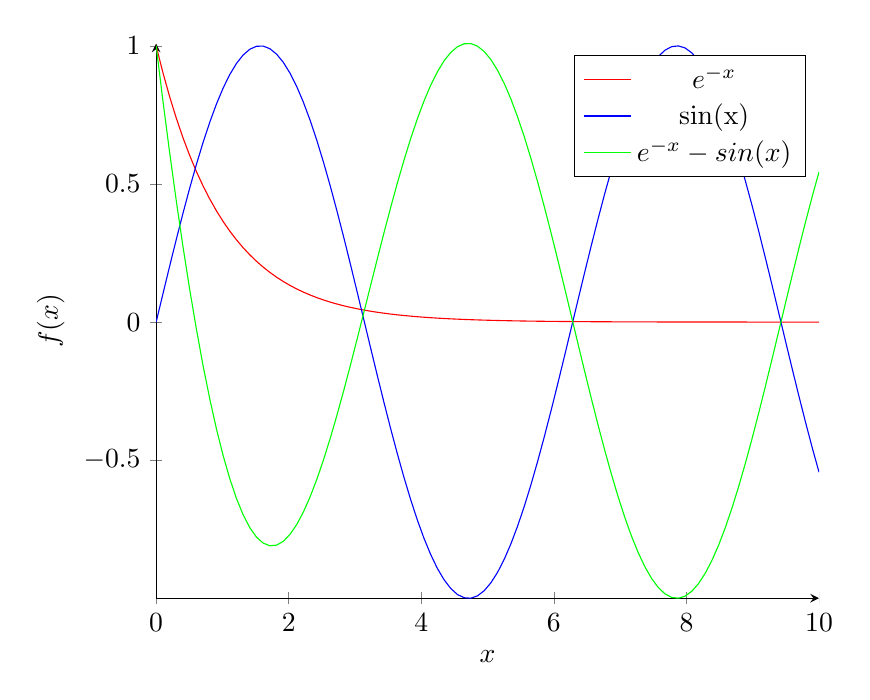
\begin{tikzpicture}
			\begin{axis}[
				axis lines = left,
				xlabel = \(x\),
				ylabel = {\(f(x)\)},
			]
			\addplot [
				domain=0:10, 
				samples=100, 
				color=red,
			]
			{e^-x};
			\addlegendentry{$e^{-x}$}
			\addplot [
				domain=0:10, 
				samples=100, 
				color=blue,
				]
				{sin(deg(x))};
			\addlegendentry{sin(x)}
			\addplot [
				domain=0:10, 
				samples=100, 
				color=green,
				]
				{e^-x-sin(deg(x))};
			\addlegendentry{$e^{-x}-sin(x)$}
			\end{axis}
			\end{tikzpicture} \\ 
			dapat dilihat bahwa untuk x $>$ 2 terdapat banyak titik potong antara ketiga fungsi tersebut
		\item Tentukan selang sehingga sehingga prosedur lelaran $x_r+1= \frac{x_r}{2} - cos(2x_r)$ konvergen di dalam selang itu (x dalam radian)
			\jaw 
			\begin{align*}
				g(x) &= \frac{x_r}{2} - cos(2x_r) \\
				g'(x) &= 2 \sin(2x_r) + \frac{1}{2} \\
			\end{align*}
			Syarat konvergen adalah $g'(x) < 1$. Jadi,
			\begin{align*}
				| 2 \sin(2x_r) + \frac{1}{2} | < 1 \\
				-1 < 2 \sin(2x_r) + \frac{1}{2} < 1 \\
				-\frac{3}{2} < 2 \sin(2x_r) < \frac{1}{2} 
			\end{align*}
			Urai satu persatu, 
			\begin{enumerate}[label=\roman*.]
				\item $2 \sin(2x_r)>-\frac{3}{2}$ memiliki nilai yang memenuhi
				\item $2 \sin(2x_r) + \frac{1}{2} < 1$ memiliki nilai yang memenuhi
			\end{enumerate}
			Maka selang agar konvergen adalah $-\frac{3}{2} < 2 \sin(2x_r) < \frac{1}{2}$ \\ \\ \\ \\ \\ \\ \\ \\ \\ \\ \\ \\ \\ \\
		\item Perlihatkan bahwa semua akar $x^{20} - 1 = 0$ berkondisi baik. \\
			\jaw
			Perhatikan graf dari fungsi $x^{20} - 1 = 0$ \\
			\begin{figure}[tph!]
				\includegraphics[width=10cm]{graph20.png}
			\end{figure} \\
			Dapat dilihat bahwa fungsi tersebut mempunyai dua akar yaitu -1 dan 1
		\item Gunakan metode \\
			(i) bagidua \\
			(ii) regula-falsi, untuk menemukan akar persaman Leonardo dalam selang [1, 1.5], dan juga
			dengan metode \\
			(iii) Newton-Raphson, x0 = 1 \\
			(iv) secant, x0=1, x1=1.5 \\
			Untuk semua metode, $\epsilon = 10^{-6}$
			\jaw 
			\[
				f(x) = x^3 + 2x^2 + 10x - 20 = 0
			\]
			\begin{enumerate}[label=\roman*.]
				\item bagidua \\
					{\small
						\begin{tabular}{ |c|c|c|c|c|c| } 
							\hline
							a&b&x&f(a)&f(b)&f(c) \\
							\hline
							1.000000000&1.500000000&1.250000000&-7.000000000&1.375000000&-3.046875000\\
							1.250000000&1.500000000&1.375000000&-7.000000000&1.375000000&-3.046875000\\
							1.375000000&1.500000000&1.437500000&-3.046875000&1.375000000&-0.900390625\\
							1.375000000&1.437500000&1.406250000&-0.900390625&1.375000000&0.220458984\\
							1.406250000&1.437500000&1.421875000&-0.900390625&0.220458984&-0.344085693\\
							1.421875000&1.437500000&1.429687500&-0.344085693&0.220458984&-0.062854766\\
							1.421875000&1.429687500&1.425781250&-0.062854766&0.220458984&0.078540325\\
							1.421875000&1.425781250&1.423828125&-0.062854766&0.078540325&0.007777512\\
							1.423828125&1.425781250&1.424804687&-0.062854766&0.007777512&-0.027554921\\
							1.424804687&1.425781250&1.425292968&-0.027554921&0.007777512&-0.009892781\\
							1.425292968&1.425781250&1.425537109&-0.009892781&0.007777512&-0.001058654\\
							1.425292968&1.425537109&1.425415039&-0.001058654&0.007777512&0.003359174\\
							1.425292968&1.425415039&1.425354003&-0.001058654&0.003359174&0.001150196\\
							1.425292968&1.425354003&1.425323486&-0.001058654&0.001150196&0.000045755\\
							1.425323486&1.425354003&1.425338745&-0.001058654&0.000045755&-0.000506453\\
							1.425338745&1.425354003&1.425346374&-0.000506453&0.000045755&-0.000230350\\
							1.425346374&1.425354003&1.425350189&-0.000230350&0.000045755&-0.000092297\\
							1.425350189&1.425354003&1.425352096&-0.000092297&0.000045755&-0.000023271\\
							1.425350189&1.425352096&1.425351142&-0.000023271&0.000045755&0.000011241\\
							1.425351142&1.425352096&1.425351619&-0.000023271&0.000011241&-0.000006014\\
							1.425351142&1.425351619&1.425351381&-0.000006014&0.000011241&0.000002613\\
							1.425351381&1.425351619&1.425351500&-0.000006014&0.000002613&-0.000001700\\
							1.425351381&1.425351500&1.425351440&-0.000001700&0.000002613&0.000000456\\
							1.425351440&1.425351500&1.425351470&-0.000001700&0.000000456&-0.000000621\\
							1.425351470&1.425351500&1.425351485&-0.000000621&0.000000456&-0.000000082\\
							1.425351470&1.425351485&1.425351478&-0.000000082&0.000000456&0.000000186\\
							1.425351470&1.425351478&1.425351474&-0.000000082&0.000000186&0.000000052\\
							1.425351474&1.425351478&1.425351476&-0.000000082&0.000000052&-0.000000015\\
							1.425351474&1.425351476&1.425351475&-0.000000015&0.000000052&0.000000018\\
							1.425351474&1.425351475&1.425351474&-0.000000015&0.000000018&0.000000001\\
							1.425351474&1.425351475&1.425351475&-0.000000015&0.000000001&-0.000000006\\
							1.425351475&1.425351475&1.425351475&-0.000000006&0.000000001&-0.000000002\\
							1.425351475&1.425351475&1.425351475&-0.000000002&0.000000001&-0.000000000\\
							1.425351475&1.425351475&1.425351475&-0.000000000&0.000000001&0.000000000\\
							1.425351475&1.425351475&1.425351475&-0.000000000&0.000000000&-0.000000000\\
							1.425351475&1.425351475&1.425351475&-0.000000000&0.000000000&0.000000000\\
							1.425351475&1.425351475&1.425351475&-0.000000000&0.000000000&0.000000000\\
							1.425351475&1.425351475&1.425351475&-0.000000000&0.000000000&0.000000000\\
							1.425351475&1.425351475&1.425351475&-0.000000000&0.000000000&-0.000000000\\
							1.425351475&1.425351475&1.425351475&-0.000000000&0.000000000&0.000000000\\
							1.425351475&1.425351475&1.425351475&-0.000000000&0.000000000&-0.000000000\\
							1.425351475&1.425351475&1.425351475&-0.000000000&0.000000000&-0.000000000\\
							1.425351475&1.425351475&1.425351475&-0.000000000&0.000000000&0.000000000\\
							1.425351475&1.425351475&1.425351475&-0.000000000&0.000000000&-0.000000000\\
							1.425351475&1.425351475&1.425351475&-0.000000000&0.000000000&-0.000000000\\
							1.425351475&1.425351475&1.425351475&-0.000000000&0.000000000&-0.000000000\\
							1.425351475&1.425351475&1.425351475&-0.000000000&0.000000000&0.000000000\\
							1.425351475&1.425351475&1.425351475&-0.000000000&0.000000000&-0.000000000\\

							\hline
						\end{tabular}
					}
				\item regula falsi \\
					{\small
						\begin{tabular}{ |c|c|c|c|c|c| } 
							\hline
							a&b&x&f(a)&f(b)&f(c) \\
							\hline
							1.0000000000&1.5000000000&1.4179104478&-0.1344081553&-7.0000000000&1.3750000000\\
							1.4179104478&1.5000000000&1.4252202700&-0.0023740705&-0.1344081553&1.3750000000\\
							1.4252202700&1.5000000000&1.4253491619&-0.0000418607&-0.0023740705&1.3750000000\\
							1.4253491619&1.5000000000&1.4253514345&-0.0000007381&-0.0000418607&1.3750000000\\
							1.4253514345&1.5000000000&1.4253514746&-0.0000000130&-0.0000007381&1.3750000000\\
							1.4253514746&1.5000000000&1.4253514753&-0.0000000002&-0.0000000130&1.3750000000\\
							1.4253514753&1.5000000000&1.4253514753&-0.0000000000&-0.0000000002&1.3750000000\\
							1.4253514753&1.5000000000&1.4253514753&-0.0000000000&-0.0000000000&1.3750000000\\
							1.4253514753&1.5000000000&1.4253514753&0.0000000000&-0.0000000000&1.3750000000\\
							1.4253514753&1.4253514753&1.4253514753&0.0000000000&-0.0000000000&0.0000000000\\
							\hline
						\end{tabular}
					}
				\item Newton Raphson \\ 
					\begin{align*}
						x_0 &= 1\\
						x_1 &= 1.6470588235294117\\
						x_2 &= 1.8285178051069293\\
						x_3 &= 1.9121971010799943\\
						x_4 &= 1.9540961957181762\\
						x_5 &= 1.9757662001654153\\
						x_6 &= 1.9871438621531745\\
						x_7 &= 1.9931625952150789\\
						x_8 &= 1.9963588018179341\\
						x_9 &= 1.9980595620433097\\
						x_10 &= 1.9989655352107734\\
						x_11 &= 1.9994484091572369\\
						x_12 &= 1.9997058533833614\\
						x_13 &= 1.9998431318038132\\
						x_14 &= 1.9999163398057687\\
					\end{align*}
				\item Secant \\ 
					\begin{align*}
						x_2 = 2.128205&\text{ }f(x_2) = 1.862725\\
						x_2 = 1.981709&\text{ }f(x_2) = -0.254747\\
						x_2 = 1.999333&\text{ }f(x_2) = -0.009333\\
						x_2 = 2.000003&\text{ }f(x_2) = 0.000049\\
						x_2 = 2.000000&\text{ }f(x_2) = -0.000000\\
					\end{align*}
			\end{enumerate}
		\item Diketahui lingkaran $x^2 + y^2 = 2$ dan hiperbola $x^2 - y^2 = 1$. Tentukan titik potong kedua kurva dengan metode lelaran titik-tetap (Soal ini adalah mencari solusi sistem persamaan nirlanjar).
			\jaw 
			Dari persamaan lingkaran, kita bisa menyatakan $y^2$ sebagai fungsi dari $x^2$: \\
			$y^2=2−x^2$

			Dari persamaan lingkaran, kita bisa menyatakan $y^2$ sebagai fungsi dari $x^2$: \\
			$y^2=x^2−1$

			Selanjutnya, dari kedua persamaan di atas, kita dapat mengeliminasi $y^2$ dengan menyetarakan kedua persamaan: \\
			$2−x^2=x^2−1$

			Gabungkan dan selesaikan persamaan berikut: 
			\begin{align*}
				x-x^2&=x^2-1 \\
				2+1&=2x^2 \\
				3&=2x^2 \\
				x^2&=\frac{3}{2} \\ 
				x &= \pm \sqrt{\frac{3}{2}}
			\end{align*}
			Untuk mencari y, substitusikan nilai $x^2=\frac{3}{2}$ ke salah satu persamaan. Misal persamaan lingkaran: 
			\begin{align*}
				y^2&=2-x^2 \\
				y^2&=2-\frac{3}{2} \\
				y^2&=\frac{1}{2} \\
				y&=\pm \sqrt{\frac{1}{2}}
			\end{align*}
			Dengan demikian, titik-titik potong kedua kurva adalah: 
			\begin{align*}
				p_1 &= \left( \sqrt{\frac{3}{2}},\sqrt{\frac{1}{2}} \right)\\
				p_2 &= \left( \sqrt{\frac{3}{2}},-\sqrt{\frac{1}{2}} \right)\\
				p_3 &= \left( -\sqrt{\frac{3}{2}},\sqrt{\frac{1}{2}} \right)\\
				p_4 &= \left( -\sqrt{\frac{3}{2}},-\sqrt{\frac{1}{2}} \right)\\
			\end{align*}
	\end{enumerate}
\end{document}
